\begin{jointwork}
	This thesis builds upon the bachelor's project `Online Marketplace Simulation: A Testbed for Self-Learning Agents' of the Enterprise Platform and Integration Concepts research group at the Hasso-Plattner-Institute. Therefore, the project will be referenced and all examples and experiments will have been conducted using its framework.
\end{jointwork}

\section{Motivation}

Nowadays, shoppers and retailers alike are getting more and more environmentally conscious. A study conducted in 2020 found that over two thirds of shoppers planned on buying sustainable clothing in the future, and over half already did buy sustainable clothing regularly~\cite{StatistaSustainableClothing}. At the same time another study reveals that retailers favour online channels over offline channels when selling used goods, with 78\% preferring the former and only 6\% the latter~\cite{StatistaUsedRetailers}. This demand is leading more and more companies, especially those selling their products through e-commerce channels, to adopt more sustainable strategies and enter the \emph{Circular Economy}, a concept we will introduce in \bfref{sec:CircularEconomy}. In the context of e-commerce, Circular Economy markets are also referred to as \emph{recommerce} markets, a phrase coined in 2005~\cite{RecommerceDefinition}.

The goal of the bachelor's project this thesis is based on was to simulate such recommerce markets, to allow for risk-free and efficient learning of market characteristics for different pricing agents. Aside from classically rule-based pricing methods, the project also focussed on training machine learning models using \emph{Reinforcement learning} (RL) algorithms on the simulated marketplace, see \bfref{sec:ReinforcementLearningIntroduction}. The focus of this thesis lies on ways that such dynamic pricing agents can be monitored and evaluated. In \cbfref{ch:RelatedWork} we will first explore the difficulties faced in dynamic pricing, as well as current and novel approaches to monitoring and evaluating RL agents in different scenarios. This will be followed by an overview of the specific features of the \emph{recommerce} market that we implemented in \cbfref{ch:SimulatingMarketplace}. In \cbfref{ch:Approaches}, we will give a detailed explanation of the different tools we built and used to monitor and evaluate our different agents. These tools will be put into context in \cbfref{ch:OurWorkflow}, where the different parts of the framework will be put to use. Finally, in \cbfref{ch:AnalysingGraphs}, we will train an RL agent using our simulation framework and take a look at how the different monitoring tools can help in evaluating its performance.

% \section*{1.2 Objective of the Thesis}

% This thesis introduces ways to monitor and evaluate different agents (rule-based as well as trained using various RL approaches) tasked with dynamically pricing products in a \emph{Circular Economy} marketplace.
% % Since the terms \emph{Reliability} and \emph{Robustness} can be interpreted differently depending on context and personal experience, we will define our usage in the \bfref{subsec:ReliabilityAndRobustness} section. Following the term definitions, we will give a short introduction and explanation of what a Circular Economy market is (\bfref{sec:CircularEconomy}) as well as what RL is and how we employ the technique in our framework (\bfref{sec:ReinforcementLearningIntroduction}).
% In this chapter, we will first introduce the general concept of a \emph{recommerce} market (\bfref{sec:CircularEconomy}) as well as \emph{RL}. In \cbfref{ch:RelatedWork} we will explore the difficulties faced in dynamic pricing and current and novel approaches to monitoring and evaluating RL agents in different circumstances. This will be followed by an overview of the specific features of the \emph{recommerce} market which we implemented in \cbfref{ch:SimulatingMarketplace}. In \cbfref{ch:Approaches} we will give a detailed explanation of the different tools we built and used to monitor and evaluate our different agents. These tools will be put into context in \cbfref{ch:OurWorkflow}, where the different parts of the framework will be put to use. Finally, in \cbfref{ch:AnalysingGraphs}, we will train an RL agent using our simulation framework and take a look at how the different monitoring tools can help in evaluating its performance.

% \subsection*{Reliability and Robustness}\label{subsec:ReliabilityAndRobustness}
% \todo{Alex: `Hast du für Reliability und Robustness irgendeine Quantifizierung? Wenn ja, und wenn die Erklärung kompakt ist würde ich die hier schon bringen.' Quantifizierung der Begriffe: Welche Metriken kommen zum Einsatz, um die jeweils zu beurteilen? Warum?}
% \begin{enumerate}
% 	\item \emph{Reliability}: With \emph{Reliability}, we describe the ability of an agent to be able to transfer knowledge of a certain type of marketplace and/or against a certain opponent over to a different scenario. If agent A performs well against agent B on marketplace M, does it perform the same against agent C on marketplace M, or against agent B on marketplace N?
% 	\item \emph{Robustness}: \emph{Robustness} is the property that describes how well an agent performs over a longer period of time. In a real-world marketplace, consistency is key to success, so finding profitability outliers and their causes are a central part of evaluating an agent's Robustness.
% \end{enumerate}

\clearpage
\section{The Circular Economy model}\label{sec:CircularEconomy}

The main goal of the aforementioned bachelor's project was to develop an online marketplace that simulates a realistic Circular Economy market environment. A market is most commonly referred to as being a \emph{Circular Economy} if it includes the three activities of reduce, reuse and recycle~\cite{circularEconomyDefinition}. This means that while in a classical Linear Economy market each product is being sold once at its \emph{new price} and after use being thrown away, in a Circular Economy, a focus is put on recycling and thereby waste reduction. In our project, we first started by modelling the simpler Linear Economy, upon which we then built the more complex Circular Economy markets. This was done by adding two additional price channels, \emph{used price} and \emph{rebuy price}, to the pre-existing \emph{new price} of a product. Refer to \Cref{fig:IntroMarketDynamics} for an overview of the product lifecycle in a Circular Economy.

\begin{figure}[t]
	\centering
	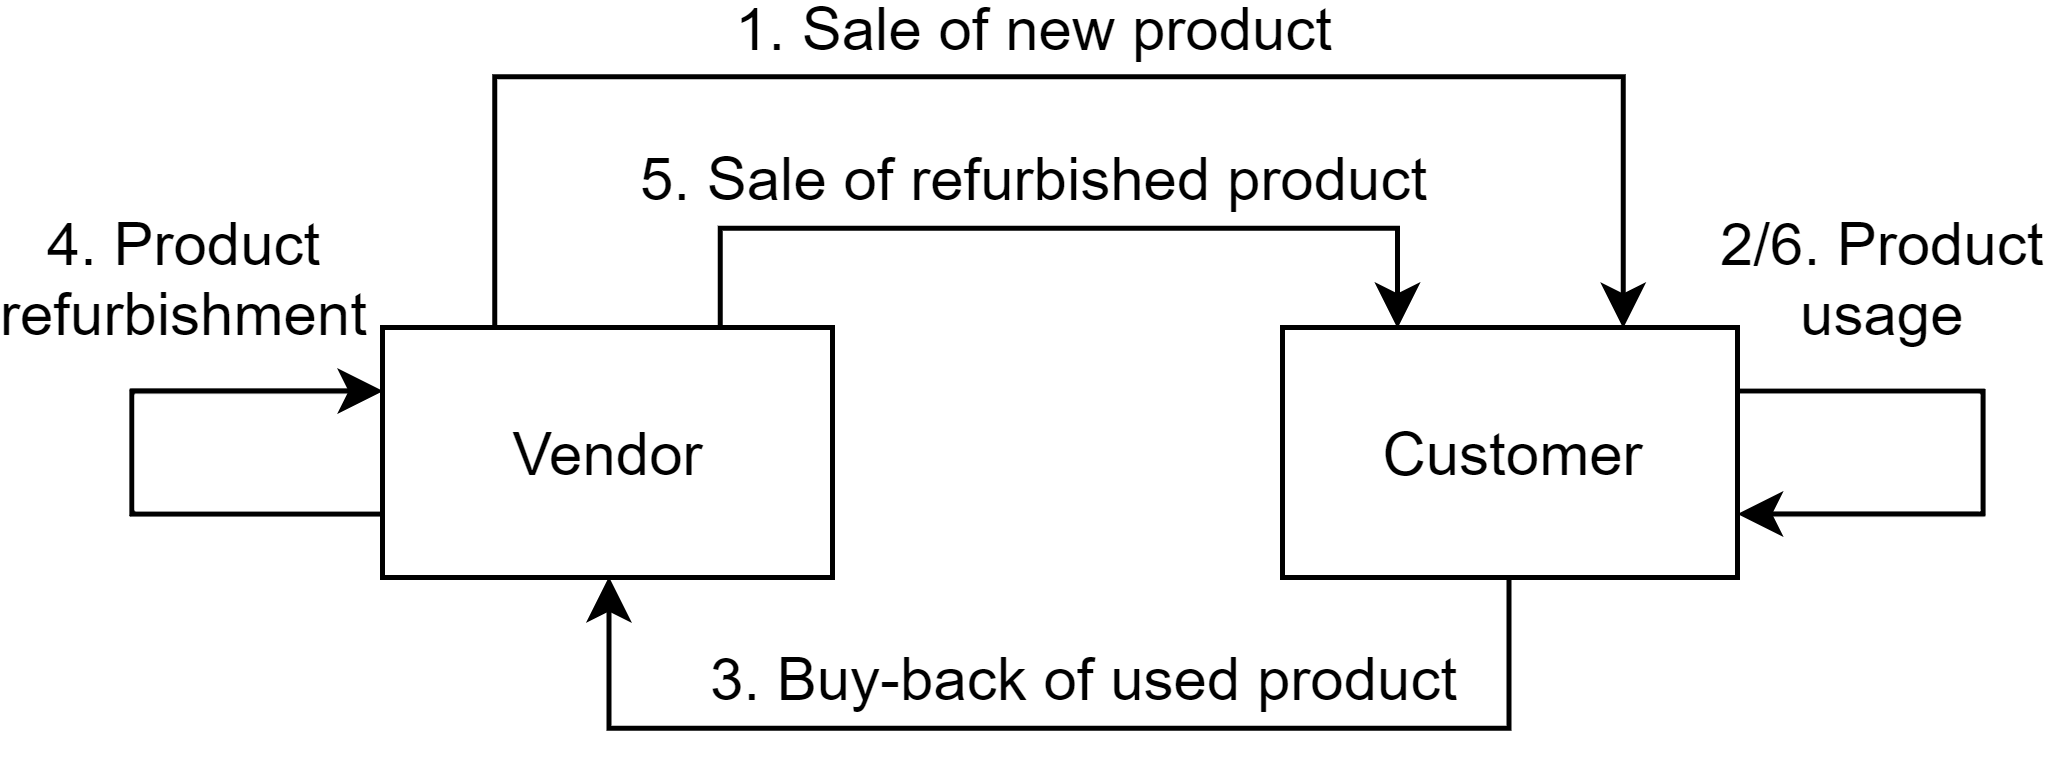
\includegraphics[width = \textwidth]{images/product_lifecycle.png}\\
	\caption{The product lifecycle in a Circular Economy (with rebuy prices). In a Linear Economy, the product lifecycle ends with step No. 2.\\ }\label{fig:IntroMarketDynamics}
\end{figure}

The \emph{rebuy price} is defined as the price a vendor is willing to pay a customer to buy back a used product, while the \emph{used price} is defined as the price the vendor sets for products they previously bought back and now want to sell alongside new products (whose price is defined by the \emph{new price}). In \bfref{sec:MarketScenarios}, we will explain the different market scenarios we modelled in more detail, together with how we transferred different aspects of these scenarios from the real market to our simulation framework. Please also refer to \Cref{fig:OverviewDiagram} for an overview of the different market components and how they interact in our framework.

From now on, when referring to a \emph{recommerce market}, we are referencing a Circular Economy marketplace with rebuy prices.

\clearpage
\section{Reinforcement learning}\label{sec:ReinforcementLearningIntroduction}

After the initial market was modelled the goal was to train agents using different RL algorithms to dynamically set prices on this marketplace, both in monopolistic scenarios and in competition with rule-based vendors which set prices following a strict set of pre-defined rules. These rules can range from simply undercutting the lowest competitor's price to more advanced techniques such as smart inventory management and reliance on previous sales data. An overview of the different types of vendors, both rule-based and using RL can be found in \bfref{sec:ExplainVendors}. Furthermore, functionality was added that allows for different RL algorithms to be trained against each other on the same marketplace, as well as functionality for so-called \emph{self-play}, where an agent plays against itself, or more precisely, against its own policy.

RL agents are trained through a process of trial-and-error. They interact with the market through an observable state and an action which influences the following state. \Cref{fig:IntroRLDiagram} illustrates the RL model in the context of our market. The goal of the agent is to maximize its \emph{reinforcement signal}, which in the case of our simulation framework is the profit the agent made during the last episode, since we want to train agents to maximize profits on real markets. An episode consists of a fixed, but pre-configurable number of time steps, where in each step each vendor (agent) sets their prices and customers make purchasing decisions. In this sense, a simulated episode could be imagined to be a day in the real world, with vendors updating their prices multiple times per day, whenever a new time step begins. By observing which prices lead to which profits (reinforcement signal), the agents get more effective in their pricing decisions over the course of training, which spans thousands of episodes in most cases.

\begin{figure}[t]
	\centering
	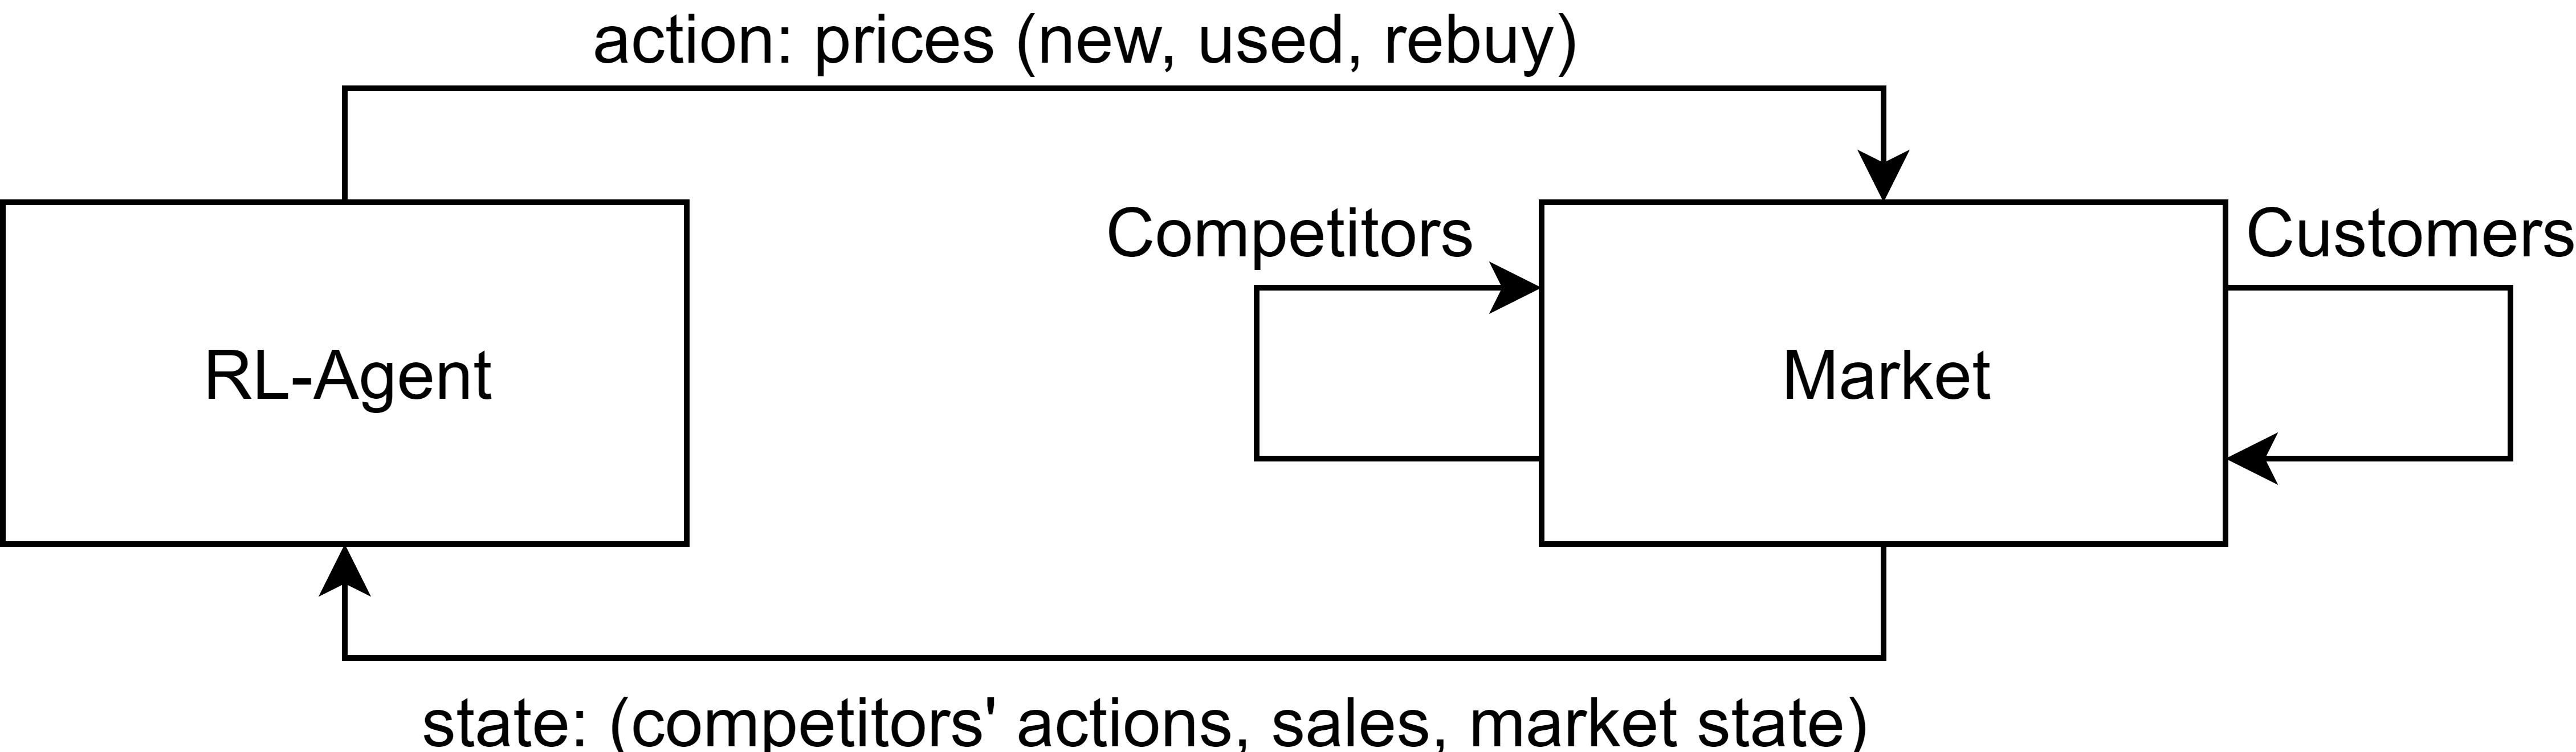
\includegraphics[width = \textwidth]{images/RL_overview.png}\\
	\caption{The standard RL model in the context of our market simulation.\\ }\label{fig:IntroRLDiagram}
\end{figure}